\documentclass{article}
\usepackage[margin=24mm]{geometry}
\usepackage{tikz}
\usepackage{hyperref}
\setlength{\emergencystretch}{3em}
\title{Hermite--Schur decoder: bounded selection campaign}
\date{Created-at: 2026-10-28 02:37 CET}
\begin{document}\maketitle
\paragraph{Acceptance.} Rebuild the supplied 883-qubit public decoder from its
hashed source and verify it with the unchanged full official DQI verifier.
Explore interchangeable jet implementations with independent value, phase and
cleanup checks. Select complete verified circuits through the existing canonical
Core/P-graph facade. Compare deterministic ordering with an actual Nagare
Chebyshev--Catmull--Rom ranker on the same candidate pool and held-out implementation
families. Report an unchanged incumbent or failed proposal honestly; improvement
and learned generalization are hypotheses, not acceptance assumptions.
\paragraph{Owners.} Transformation's Quantum package owns the domain adapter,
candidate contracts and derived circuit features. Existing Core/Query and P-graph
own parsing, canonical identity and ABB selection. The supplied Apache-2.0
notebook source remains a hash-bound external generator, with attribution and
without edits to its snapshot. Nagare's existing Python Plan/train/forward facade
owns training; Tensor owns Chebyshev/CR evaluation. Consume the existing native
binary in a separate process and record its hash: its source revision is unproven.
No training loop, spline kernel, verifier, parser or graph search is copied here.
Nagare's provider-pin mismatch is outside scope; no Nagare repository changes.
\paragraph{Checkout and discovery.} Reuse Transformation feat/unversioned at
32c6bb3, current with both fetched remotes. Preserve all unrelated dirty files.
Existing quantum adapters, selectors, budget supervisor and public source were
inspected. No manifest or protected-file changes. No new worktree, commit, push,
Kaggle submission, host service change or WSL execution.
\paragraph{Experiment.} First reproduce the exact baseline binary. Then enumerate
forward/reverse jet pairs (pro, narrow, original), check semantic compatibility
including zero inputs and deferred measurement phases, and measure native resources.
Screen full-context workspace/Toffoli estimates before expensive full builds.
Test a bounded set of promising integrated variants, retaining baseline as control.
Learning uses training-only feature scaling and family-held-out evaluation; known
exact costs remain the deterministic control, never hidden to fabricate a gain.
If the finite pool is too small to support learning conclusions, label the result
a wiring experiment and retain the measured incumbent.
\paragraph{Budgets and ETA.} Amaterasu, pinned Python 3.13 image and existing
read-only official runtime. One CPU, no network inside experiment containers.
At most one large job: 10 GiB sampled RSS / 12 GiB hard container limit and
900 seconds per build or verifier. Small kernel campaign: 2 GiB, 900 seconds.
Learning: one CPU, 2 GiB, 300 seconds. At most four full variants after baseline,
one fixed local verification salt, no salt tuning. ETA 60--90 minutes plus the
existing report archive scan. Durable command/resource/status receipts at each stage.
\paragraph{Evidence.} Source and artifact SHA-256, original notebook attribution,
kernel contracts, failures, native counts, full verifier results and resource logs.
Score uses measured global peak qubits and mean executed Toffolis, with the official
error repetition factor. Microkernel cost is not a full decoder score. Learned
ordering never establishes validity or an admissible ABB lower bound.
\paragraph{Rollback and close.} New task-owned paths only; preserve old circuits
and source snapshots. Consolidate one report and archive once after writers stop.
\paragraph{Implemented interfaces and files.} No protected items were touched.
Quantum Python adds \texttt{hermite.py} (hash-bound library, phase-token adapters,
kernel checks and live-workspace dispatch) and \texttt{proposal\_ranker.py}
(Nagare facade experiment). Tools adds \texttt{quantum\_hermite.py},
\texttt{quantum\_ranker.py}, and \texttt{test\_quantum\_hermite.py}; extends
\texttt{quantum\_views.py}, \texttt{report.py}, and the Quantum/tool READMEs.
No Rust public API or dependency changes. Actual large jobs: baseline build,
baseline verification, adaptive 883 build, adaptive 879 build and verification,
serialized. The adaptive 883 build reproduced the control bytes exactly.
The KAN experiment uses the existing Nagare native Python module, six training
kernel pairs and three pairs from a held-out forward implementation. It establishes
integration only; it does not establish faster full-circuit search.
\begin{center}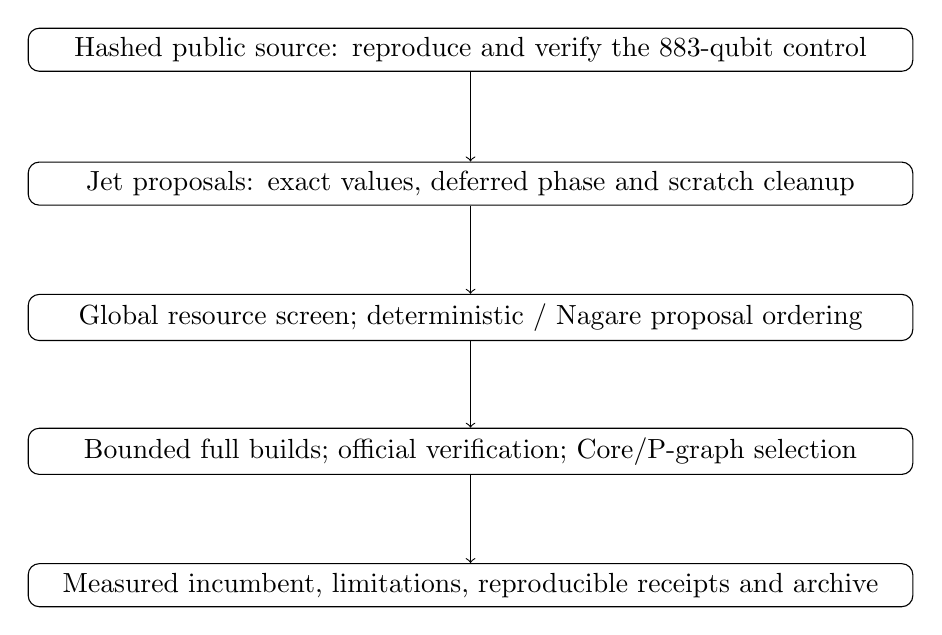
\begin{tikzpicture}[every node/.style={draw,rounded corners,align=center,text width=11cm},node distance=17mm]
\node (a) {Hashed public source: reproduce and verify the 883-qubit control};
\node (b) [below of=a] {Jet proposals: exact values, deferred phase and scratch cleanup};
\node (c) [below of=b] {Global resource screen; deterministic / Nagare proposal ordering};
\node (d) [below of=c] {Bounded full builds; official verification; Core/P-graph selection};
\node (e) [below of=d] {Measured incumbent, limitations, reproducible receipts and archive};
\draw[->] (a)--(b); \draw[->] (b)--(c); \draw[->] (c)--(d); \draw[->] (d)--(e);
\end{tikzpicture}
\end{center}
\end{document}
